\documentclass[12pt]{article}
\usepackage{fontspec}
\usepackage{xeCJK}
\usepackage{xcolor}
\usepackage[a4paper, margin=2cm]{geometry}
\usepackage{setspace}
\usepackage{indentfirst}
\usepackage{tcolorbox}
\usepackage{graphicx}
\usepackage[stable]{footmisc}
\usepackage{hyperref}
\usepackage{csvsimple}
\usepackage{float}
\usepackage{subcaption}

\hypersetup{
    colorlinks=true,
    linkcolor=blue,
    filecolor=magenta,      
    urlcolor=cyan,
}
 
\urlstyle{same}

\graphicspath{ {./images/} }

\onehalfspacing
\definecolor{friendlybg}{HTML}{f0f0f0}

\setCJKmainfont{Noto Serif CJK SC}
\setCJKmonofont{Noto Sans CJK SC}
\setromanfont{Noto Serif Regular}
\setsansfont{Noto Sans Regular}
\setmonofont{Fira Code}[
  Contextuals=Alternate  % Activate the calt feature
]
\usepackage{listings}
\usepackage{lstfiracode}

\definecolor{friendlybg}{HTML}{f0f0f0}
\ActivateVerbatimLigatures

\title{程序设计实践大作业设计报告}
\author{2020211659 滕宇航}
\date{November, 2022}

\newenvironment{aside}[1]
    { \begin{tcolorbox}[enlarge top by=0.5cm, enlarge bottom by=0.5cm] Aside\space\space\space\space \textbf{#1} \\
        } { \end{tcolorbox} }
        
\renewcommand{\figurename}{图}
\renewcommand{\tablename}{表}

\begin{document}

\maketitle 

    在过去的两个星期里,我用 Rust 语言实现了一个领域内特定脚本语言的解释器,该解释器支持个人自定义的脚本文法。本文将介绍文法的定义方式和解释器的实现思路,以及在实现过程中我是如何完成作业要求的。

    \section{为什么使用 Rust?}

    Rust 语言相比于其他诸如 C,C++,java 等语言的一个巨大优势是该语言的各种现代化特性,比如:

    \begin{enumerate}
        \item 强大的包管理工具和配置工具 cargo,C++ 语言生态一直没有一个通用且简洁的包管理工具。
        \item 内置单元测试和集成测试,而且通过 cargo 可以自动运行所有测试桩,不用找其他工具进行额外配置。
            \begin {aside}{项目内的一个单元测试示例,源自\href{../src/scanner.rs}{scanner.rs}}
                \begin{verbatim}
    #[test]
    fn test_scan_tokens_keywords() {
        let source = "true false".to_string();
        let mut scanner = Scanner::new(source);
        let tokens = scanner.scan_tokens();
        assert_eq!(tokens.len(), 2);
    }
                \end{verbatim}
            \end {aside}
        \item 多种模式的注释,有专用的文档注释,通过 cargo 命令可以直接生成文档注释嵌入的程序模块文档和程序间接口文档,使得理解 rust 项目逻辑变的更加容易。
        \item 严格的编译期管理和检查,对于每个不符合 rust 代码风格要求的地方都会报 warning 来提醒你改善代码,使得该项目代码有着良好的风格。
    \end{enumerate}

    基于上述特性,在达成作业要求时使用 rust 语言是一个好的选择。


    \begin{aside}{ rust 的上述特性是如何应用到该项目中的?}
        \begin{enumerate}
        \item 风格方面,通过 cargo check 命令可以检查项目的代码风格是否满足 rust 对风格的要求,在编译时也会对风格和要求不一致的地方做出提醒;通过 cargo doc 命令可以根据注释生成项目各模块的文档。
        \item 接口方面,通过代码的文档注释和 cargo doc 命令可以生成程序间接口的文档,参考\href{generate_by_cargo/robot_dsl/index.html}{文档}。
        \item 测试方面,每个模块都有相关的单元测试(在每个模块文件的最底部),因依赖别的模块而无法单独单元测试的有专门的集成测试(tests 文件夹),运行 cargo test 可以自动运行所有的测试桩。
        \end{enumerate}
    \end{aside}

    \section{脚本文法介绍}

    我在定义脚本语言语法时使用了和一般 BNF 范式略有不同的一套记法,方便我理解语法和根据语法写解析程序。以下介绍脚本语言语法的语法规则和记法。

    \subsection{符号说明}

    \begin{itemize}
        \item 终止符:带引号的符号,例如"true",表示文法在这里终止。
        \item 非终止符:不带引号的符号,例如 expression,非终止符在脚本语言文法中有递归的含义。
        \item“|”:管道符,分割开两种不同的记法,表示该非终止符,可以被两种具有或关系的记法表示。
        \item“(”“)”:分组,将括号内的符号一起解析。
        \item“*”:和 BNF 范式的意义一样,表示可以重复多次被“*”标记的符号组。
        \item“?”:该标记可以不存在,可以重复多次。
    \end{itemize}

    \subsection{总的文法规则}

    在这里我将采用递归下降的方式来介绍文法的规则,首先是大致的文法框架:

    \begin{verbatim}
        program     -> declaration* EOF;
        declaration -> vardec | stepdec | statement
        statement   -> exprStat | speakStat | 
                       listenStat | inputStat |
                       inputnStat | exitStat |
                       blockStat | branchStat | loopStat
    \end{verbatim}

    由符号意义以及文法规则可以看出,脚本程序由声明和终止符组成,声明分为变量声明,函数声明和语句三类。下面先介绍语句相关的文法,变量声明参考\ref{vars},函数声明参考\ref{func}。

    \subsection{语句的定义规则}

    语句一共有两类:核心语句和辅助语句。再介绍这两类语句之前,还需要介绍构成语句的一个重要元素:表达式。

    \subsubsection{词法分析和表达式分析}

    当解释器扫描脚本时,解释器做的第一件事是对脚本的词素进行扫描和词法分析,对词素所分的类别参考\href{generate_by_cargo/robot_dsl/token/enum.TokenType.html}{相关文档}。

    对词素进行分类后即可进行表达式相关的分析,表达式相关文法如下:

    \begin{verbatim}
        expression -> assignment
        assignment -> IDENTIFIER "=" assignment | equality
        equality   -> term ("!="|"==") term
        term       -> unary ("-"|"+") unary
        unary      -> "!" unary | call
        call       -> primary ("(" arguments? ")" )*
        arguments  -> expression (","expression)*,
        primary    -> NUMBER | STRING | IDENTIFIER 
                      | "true" | "false" 
                      | "Nil" | "expression"   
        NUMBER     -→ DIGIT+ ( "." DIGIT+ )? ;
        STRING     -→ "\"" <any char except "\"">* "\"" ;
        IDENTIFIER -→ ALPHA ( ALPHA | DIGIT )* ;
        ALPHA      -→ "a" ... "z" | "A" ... "Z" | "_" ;
        DIGIT      -→ "0" ... "9" ;
    \end{verbatim}

    表达式文法只需按照递归下降的逻辑理解即可,具体解释参考\href{generate_by_cargo/robot_dsl/syntax/enum.Expr.html}{相关文档}。需要注意的是为了契合脚本语言的实际应用场景,表达式并未递归分析太多的运算符和优先级等问题,最多支持二元相关的计算。

    \subsubsection{核心语句}

    核心语句即一般的编程语言常见的块语句,表达式语句,分支语句和循环语句,文法规则如下:

    \begin{verbatim}
        expressionStat -> expression ";"
        blockStat      -> "{" dec* "}";
        branchStat     -> "branch" "(" expression ")" statement
        loopStat       -> "loop" statement
    \end{verbatim}

    \subsubsection{辅助语句}

    由于个人设计的脚本语言没有一般语言对于为了支持输入输出等功能而设计的相关库函数,所以我添加了一些和输入输出等功能相关的辅助语句来扩展脚本语言支持的操作,辅助语句分为如下五种:

    \begin{itemize}
        \item 输出语句:输出表达式值
        \item 输入字符串语句:输入字符串,定义字面值为变量,将字符串赋值给变量
        \item 输入数字语句:功能类似于输入字符串语句
        \item 等待语句:等待多少秒
        \item 退出语句:退出脚本程序
    \end{itemize}

    相应文法规则如下:

    \begin{verbatim}
        speakStat  -> "speak" expression ";"
        inputStat  -> "input" IDENTIFIER ";"
        inputnStat -> "inputn" IDENTIFIER ";"
        listenStat -> "listen" expression ";"
        exitStat   -> "exit"
    \end{verbatim}

    \subsection{变量和函数的定义规则}\label{vars}

    若要定义一个变量首先要有支持该变量的运行时环境,其次要有赋值表达式来支持对变量的赋值;定义函数同理,需要函数的运行时环境和函数调用相关的表达式。以下是变量声明和函数声明的相关文法,

    \begin{verbatim}
        vardec -> "var" IDENTIFIER ("="expression)?";"
        stepdec   -> "step" function
        function  -> IDENTIFIER "(" parameter? ")" blockStat
        parameter -> IDENTIFIER ("," IDENTIFIER)*
    \end{verbatim}
    
    \section{解释器的实现思路}

    \subsection{模块划分和功能实现过程}\label{mod}

    \begin{figure}[h]
        \centering
        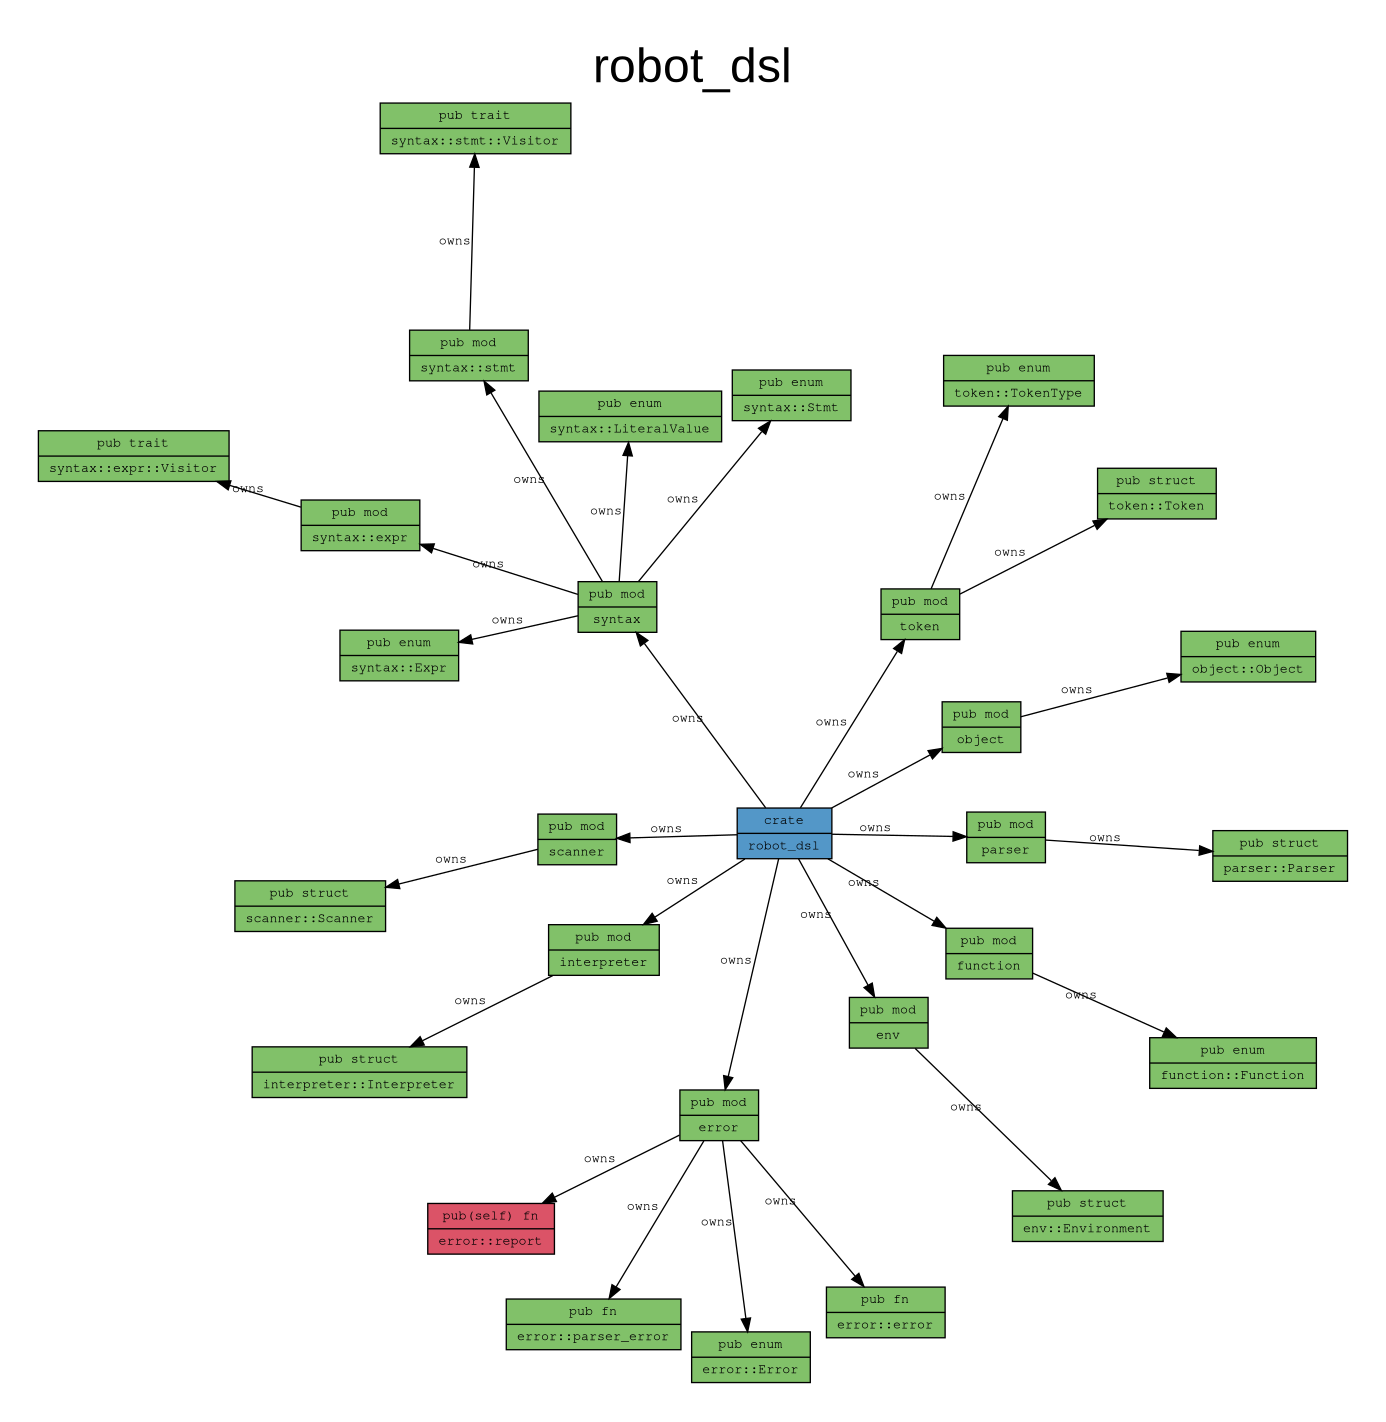
\includegraphics[width=0.9\textwidth]{mod-graph.png}
        \caption{模块图}
        \label{fig:mod-graph}
    \end{figure}

    模块图如图\ref{fig:mod-graph}所示,具体模块解释和相关接口参考\href{generate_by_cargo/robot_dsl/index.html}{文档}。

    下面通过一段代码说明各模块间是如何合作达到解析脚本语言的过程的(摘自\href{../src/main.rs}{main.rs})。:

    \begin{verbatim}
        let mut scanner = Scanner::new(source);
        let tokens = scanner.scan_tokens();
        let mut parser = Parser::new(tokens);
        let statements = parser.parse()?;
        self.interpreter.interpret(&statements)?;
    \end{verbatim}

    由代码可知,解释器先调用 scanner 模块对脚本代码的词素进行扫描和分析后,再 调用 parser 模块进行解析,最后调用 interpreter 模块进行解释,从而实现解释器的功能。

    \subsection{数据结构介绍}

    \subsubsection{核心数据结构}

    由\ref{mod}可知,核心模块即 \href{generate_by_cargo/robot_dsl/scanner/struct.Scanner.html}{scanner}, \href{generate_by_cargo/robot_dsl/scanner/struct.Parser.html}{parser}, \href{generate_by_cargo/robot_dsl/scanner/struct.Interpreter.html}{interpreter} 三大部分。但是这三者共同作用于一个核心数据结构:\href{generate_by_cargo/robot_dsl/syntax/enum.Stmt.html}{statement}。

    statement 通过 rust 特有的\href{https://doc.rust-lang.org/stable/reference/items/enumerations.html}{枚举类型}和句法分析中递归下降分析的思路来定义了一个语法树,相关的文法规则上面已经有了介绍。statement 枚举了所有的脚本语法的语句类型,在不同函数中匹配 statement 中所定义的不同类型,从而逐层递归,解析出了脚本的语法树。

    \begin{aside}{visitor 模式}
        scanner 和 parser 模块的结合显而易见,但是 parser 和 interpreter 的结合借鉴了一个经典的设计模式:visitor 模式。百度百科的定义是表示一个作用于某对象结构中的各元素的操作。它使你可以在不改变各元素类的前提下定义作用于这些元素的新操作。这里通过 \href{https://doc.rust-lang.org/stable/reference/items/traits.html}{trait} 语法来实现 visitor 模式,从而使 interpreter 可以访问 statement 结构并进行相关操作,进而和 parser 模块进行交互。
    \end{aside}

    \subsubsection{周边数据结构}

    为了支持变量的定义和运行,解释器需要执行环境相关的\href{generate_by_cargo/robot_dsl/env/index.html}{数据结构}来保障脚本的正常运行。

    为了支持脚本语法的错误处理,解释器需要语法错误处理相关的\href{generate_by_cargo/robot_dsl/error/index.html}{数据结构}。

    为了支持函数环境的嵌套,解释器需要函数相关的\href{generate_by_cargo/robot_dsl/function/index.html}{数据结构}来处理不同函数的作用域和函数调用问题。为了契合实际,脚本语法不支持处理递归函数等复杂的作用域场景处理。


\end{document}
